%%%%%%%%%%%%%%%%%%
% Based on https://github.com/jdavis/latex-homework-template
%%%%%%%%%%%%%%%%%%

\documentclass{article}

\usepackage{fancyhdr}
\usepackage{extramarks}

\usepackage{amsmath}
\usepackage{amsthm}
\usepackage{amsfonts}

\usepackage{tikz}
\usepackage[plain]{algorithm}
\usepackage{algpseudocode}

\usepackage{lipsum}

%for urls
\usepackage{hyperref}
\hypersetup{
	colorlinks = true,
	linkcolor = teal,
	anchorcolor = teal,
	citecolor = teal,
	filecolor = teal,
	urlcolor = teal
}

%%%%%% Basic Document Settings %%%%%%%%%

\topmargin=-0.45in
\evensidemargin=0in
\oddsidemargin=0in
\textwidth=6.5in
\textheight=9.0in
\headsep=0.25in

\linespread{1.1}

%%%%%%%%%%%%%%%%%% Homework Details %%%%%%%%%%%%%%%
% Title
% Due date
% University
% Class
% Instructor
% Author
% Author ID 

\newcommand{\hmwkTitle}{Assignment\ \#2}
\newcommand{\hmwkDueDate}{Nov 13, 2022}
\newcommand{\hmwkClass}{Introduction to Artificial Intelligence (CS-487)}
\newcommand{\hmwkClassInstructor}{Professor I. Tsamardinos}
\newcommand{\hmwkUniversity}{University of Crete \\Department of Computer Science}
\newcommand{\hmwkAuthorName}{Nikolaos Kougioulis}
\newcommand{\hmwkAuthorID}{ID 1285}


\pagestyle{fancy}
\lhead{\hmwkAuthorName\ (\hmwkAuthorID)} %left head
%\chead{\hmwkClass\ \hmwkTitle} %center head
%\rhead{\date{\today}} %right head
\rhead{\hmwkClass\ \hmwkTitle} 
\lfoot{\lastxmark}
\cfoot{\thepage}

\renewcommand\headrulewidth{0.4pt}

\setlength\parindent{0pt}

\setcounter{secnumdepth}{0}
\newcounter{partCounter}
\newcounter{ExerciseCounter}
\setcounter{ExerciseCounter}{1}
\nobreak\extramarks{Exercise \arabic{ExerciseCounter}}{}\nobreak{}

%%%%%% Homework Problem Environment %%%%%%
\newenvironment{Exercise}[1][-1]{
	\ifnum#1>0
	\setcounter{ExerciseCounter}{#1}
	\fi
	\section{Exercise \arabic{ExerciseCounter}}
	\setcounter{partCounter}{1}
}{
}
% Alias for the Solution section header
\newcommand{\solution}{\textbf{\large Solution:}}

% Title Page %
\title{
	\centering
	
\includegraphics[height=1.5in]{images/background.png}
	
	 \vspace{1in}
	\textmd{\textbf{\hmwkClass\ \hmwkTitle}}\\
	
	\normalsize\vspace{0.1in}\small{Due\ on\ \hmwkDueDate}\\
	
	\vspace{0.1in}
	\large{\textit{\hmwkClassInstructor}} \\
	\vspace{0.5in}
	
	\large{\hmwkUniversity}

	\vspace{3in}
	
	\author{\textbf{\hmwkAuthorName} (\hmwkAuthorID)}
	\date{\today}
}

% Various Helpers %
\newcommand{\alg}[1]{\textsc{\bfseries \footnotesize #1}}
% For derivatives
\newcommand{\deriv}[1]{\frac{\mathrm{d}}{\mathrm{d}x} (#1)}
% For partial derivatives
\newcommand{\pderiv}[2]{\frac{\partial}{\partial #1} (#2)}
% Integral dx
\newcommand{\dx}{\mathrm{d}x}
\newcommand{\E}{\mathbb{E}}
\newcommand{\Var}{\mathrm{Var}}
\newcommand{\Cov}{\mathrm{Cov}}
\newcommand{\Bias}{\mathrm{Bias}}

%\def\blankpage{%
%	\clearpage%
%	\thispagestyle{empty}%
%	\addtocounter{page}{-1}%
%	\null%
%	\clearpage}


%for code listings
\usepackage{listings}
\usepackage{xcolor}

\definecolor{codegreen}{rgb}{0,0.6,0}
\definecolor{codegray}{rgb}{0.5,0.5,0.5}
\definecolor{codepurple}{rgb}{0.58,0,0.82}
\definecolor{backcolour}{rgb}{0.99,0.99,0.99}

\lstdefinestyle{mystyle}{
	backgroundcolor=\color{backcolour},   
	commentstyle=\color{codegreen},
	keywordstyle=\color{magenta},
	numberstyle=\tiny\color{codegray},
	stringstyle=\color{codepurple},
	basicstyle=\ttfamily\footnotesize,
	breakatwhitespace=false,         
	breaklines=true,                 
	captionpos=b,                    
	keepspaces=true,                 
	numbers=left,                    
	numbersep=5pt,                  
	showspaces=false,                
	showstringspaces=false,
	showtabs=false,                  
	tabsize=2
}

\lstset{style=mystyle}

%ONLY FOR THIS DOCUMENT!
%Concerning Exercise 4
\renewcommand{\figurename}{\textbf{Solution} to Question}

\begin{document}

	\maketitle
	
	%\blankpage
	
	%\setcounter{page}{1}
	\begin{Exercise}[1]
		Give the name of the algorithm that results from each of the following special cases:
		\begin{enumerate}
			\item Local beam search with $k=1$.
			\item Local beam search with one initial state and no limit on the number of states retained.
			\item Simulated annealing with $\mathrm{T}=0$ at all times (and omitting the termination test).
			\item Genetic algorithm with population size $\mathrm{N}=1$.
		\end{enumerate} \vspace{6pt}
	
		\solution \\
		
		\begin{enumerate}
			\item Local Beam Search with $k=1$ keeps track of only one state, so it represents \textit{Hill-Climbing}. 
			\item Local Beam Search with one initial state and no limit on the number of states retained results in \textit{Breadth-First Search}, as the algorithm expands the frontier.
            \item Simulated annealing with $\mathrm{T} = 0$ selects the first next state with the optimal $\Delta x$ so it resembles \textit{Best-First Hill-Climbing}. % because every downward successor will be rejected with probability 1.
            \item A Genetic Algorithm with population size $\mathrm{N} = 1$ performs a (trivial) selection on the single individual of the population, the two parents are the same, which then results in the same crossover and a random mutation, so it results in a \textit{random walk}\footnote{\url{https://mathworld.wolfram.com/RandomWalk1-Dimensional.html}} ( or a \textit{Brownian motion}\footnote{\url{https://mathworld.wolfram.com/BrownianMotion.html}} in the case of continuous time and space) with probability equal to the mutation rate.
		\end{enumerate}
		
	\end{Exercise}

    \newpage

    \begin{Exercise}[2]
     		Which of the following are true and which are false? Give brief explanations.
     		\begin{enumerate}
     			\item In a fully observable, turn-taking, zero-sum game between two perfectly rational players, it does not help the first player to know what strategy the second player is using—that is, what move the second player will make, given the first player’s move.
     			\item A perfectly rational backgammon agent never loses. \\
     		\end{enumerate}
     	
     	\solution \\
        \begin{enumerate}
            \item \textbf{False}. In a fully observable, turn-taking, zero-sum game is it optimal to know the strategy of the opponent. This statement would be true in the case of a \textbf{\textit{partially}} observable, turn-taking, zero-sum game.
            \item \textbf{False}. Backgammon is a \textbf{\textit{stochastic}} game, so even a perfectly rational agent may lose, due to the factor of stochasticity involved in rolling a die (or dice). Success in the game does not only depend on the agent's skill, but also on pure luck.
        \end{enumerate}
     	
    \end{Exercise}

    \newpage

    \begin{Exercise}[3]
    	Discuss how well the standard approach to game playing would apply to games such as tennis, pool, and croquet, which take place in a continuous physical state space. \\
    	
    	\solution \\
    	
    	%The issue here is that instead of a discrete, fully observable state space we are faced with a continuous physical state space. 
    	One way to approach these problems,discussed in Chapter 4, is to discretize the continuous state space, based on a spacing of size $\epsilon$. \\
    	
    	In the case of tennis, by discretizing states such as the speed of the racket hit and the positioning of the ball one may yield average results. One may perform Minimax for alternating turns of ball direction (left opposite corner, middle, right opposite corner) and ball speed (low,medium,fast), or even ExpectMiniMax after performing a Monte Carlo simulation to deduce the necessary probability distributions. \\
    	
    	But in the case of pool and croquet, such approach must be mediocre at best. Both pool (8-ball pool or snooker) and croquet are sports that require great amounts of accuracy, with very small differences between a winning and a losing state; the positioning of the mallet, the balls and the hoops (not even taking into consideration the anomalies on the grass surface), as well as the positioning of the cue and the balls, are highly complex environments that will suffer from discretization techniques. \\
    	
    	However one can consider individual tasks using local search in continuous spaces (\textit{Chapter 4, Section 2}). For example, in 8-ball pool the goal of winning consists of potting all single color (or striped) balls and the 8-ball last. A local-search algorithm (like the empirical gradient method or Newton-Raphson's method) can indeed find the optimal way to achieve every local goal like "run the hoop", "play the correct ball" for croquet\footnote{\url{https://www.croquet.org.uk/?p=games/garden/rules/GardenGolfRules}} or "break the rack", "pot ball numbered k", "pot the 8-ball"\footnote{\url{https://upatour.com/8-ball-rules/}}, which are definitely more approachable methods than trying to learn an agent how to play human-like tennis in a continuous environment.
    	
    \end{Exercise}

    \newpage
    
    \begin{Exercise}[4]
     	\begin{enumerate}
     		\item  Give the values calculated by Minimax for all states in the tree. Do not use alpha-beta pruning.
     		\item Indicate which branches of the tree will be pruned by alpha-beta pruning.
     	\end{enumerate}
     
     \begin{figure}
     \centering
     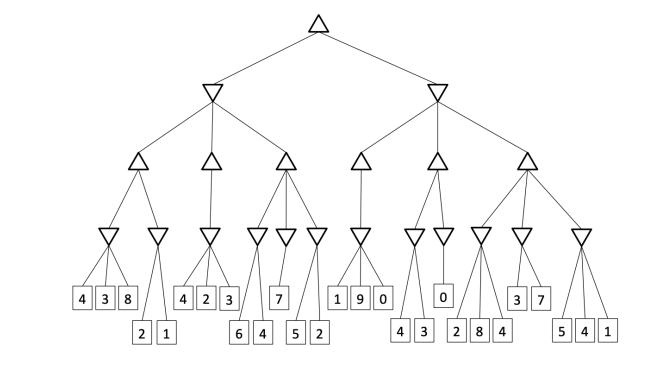
\includegraphics[width=1.0\textwidth]{images/tree.png}
     \end{figure}
     \vspace{6pt}
     
     
          \solution \\
          
          \textit{Continued on next page...}
          
              \begin{figure}
              	\centering
              	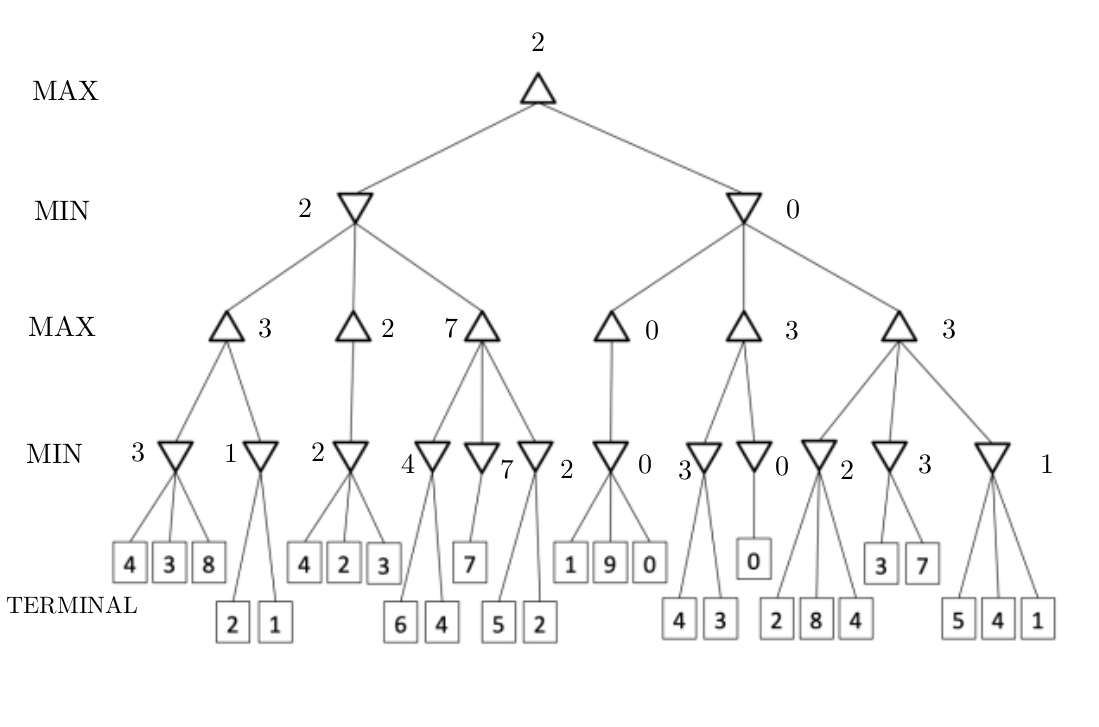
\includegraphics[width=0.8\textwidth]{images/minmax.png}
              	\caption{Application of Minimax for all states of the tree, calculated iteratively from the terminal states to the root state. Minimax performs a complete depth-first exploration of the game tree. If there are $b$ legal moves at each point and the depth of the tree is $m$, then the time complexity of Minimax is $\mathcal{O}(b^m)$ and the space complexity $\mathcal{O}(bm)$ respectively.}
              \end{figure}
          
              \begin{figure}
              	\centering 
              	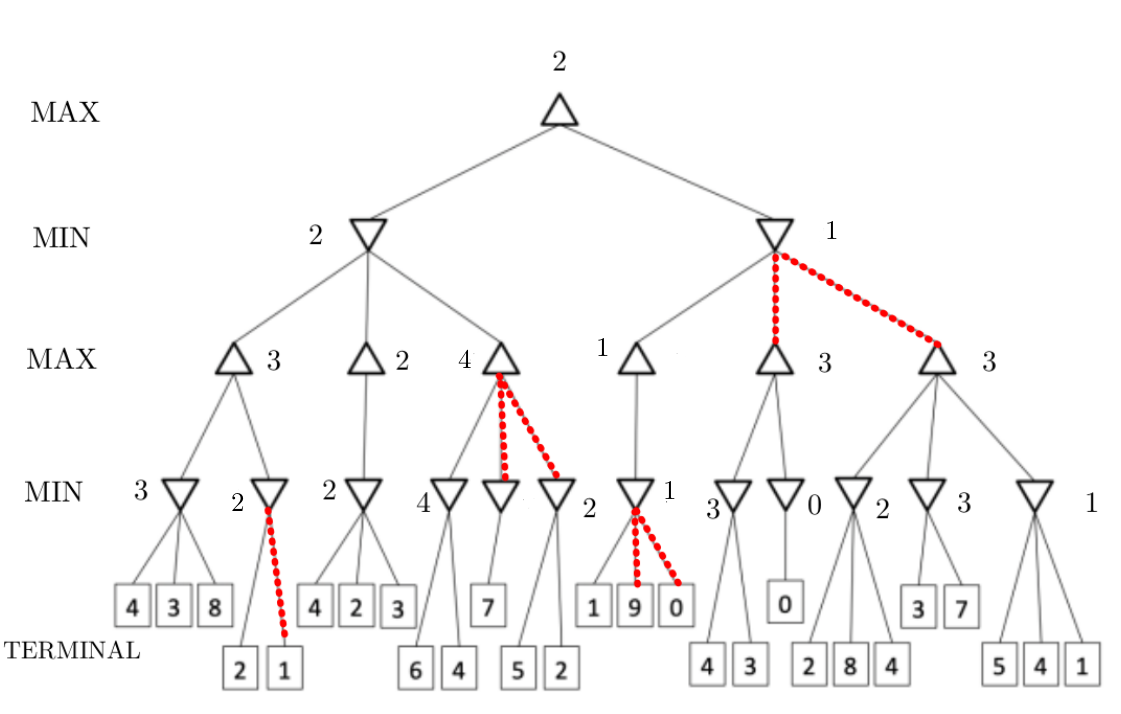
\includegraphics[width=0.8\textwidth]{images/alpha_beta_pruning.png}
              	\caption{Due to the exponential complexity of the Minimax algorithm, it is viable to find the actual Minimax decision without even looking at every node of the game tree, using alpha-beta pruning. By applying alpha-beta pruning to the Minimax algorithm, the sames moves get returned but nodes that are possibly not affecting the final decision are removed (pruned) from the search tree. } 
              \end{figure}
          
     \end{Exercise}

\end{document}
